%-----------------------------------------
% Note: Use pdflatex to process this file.
%-----------------------------------------

\documentclass{book}

%%\usepackage[all]{nowidow}
\usepackage{index}
\usepackage{setspace}
\usepackage{graphicx}
\usepackage{moreverb}    % Defines {listing} environment.
\usepackage{amsmath, amsthm, amssymb, amsbsy, mathtools}
\usepackage{alltt}
\usepackage{rotating}
\usepackage{subcaption}
\usepackage{xspace}
\usepackage{xcolor}
%%\usepackage{makeidx}
\usepackage[section]{placeins}   % For preventing floats from floating to end of chapter.
\usepackage{longtable}  % For splitting long vertical tables into pieces
\usepackage{multirow}
\usepackage{booktabs}   % For table layouts
\usepackage{yhmath}     % For widehat
\usepackage{eso-pic}    % For cover graphics
\usepackage{enumitem}
%%\usepackage{fancyvrb}

\usepackage[T1]{fontenc}   % so _, <, and > print correctly in text.
\usepackage[strings]{underscore}    % to use "_" in text
\usepackage[pdftex,colorlinks=true,bookmarksnumbered=true]{hyperref}   % Must be last package!

%----------------------------------------------------------------
\input{macros.tex}

\setlength{\textwidth}{6.25in}
\setlength{\hoffset}{0.0in}
\setlength{\oddsidemargin}{0.25in}
\setlength{\evensidemargin}{0.0in}
\setlength{\textheight}{8.5in}
\setlength{\topmargin}{0in}

\renewcommand{\textfraction}{0.1}
\renewcommand{\topfraction}{1.0}
\renewcommand{\bottomfraction}{1.0}

\begin{document}

%----------------------------------------------------------------

\thispagestyle{empty}

\raisebox{-0.8in}{
\includegraphics[width=2in]{scibmad.pdf}}
\hfill
\parbox[b]{1.8in}{\large
  Date: 2024-10-3 \\
  Version: 0.5.5
}

\pdfbookmark[0]{Preamble}{Preamble} 

\vfill

{
\begin{center}
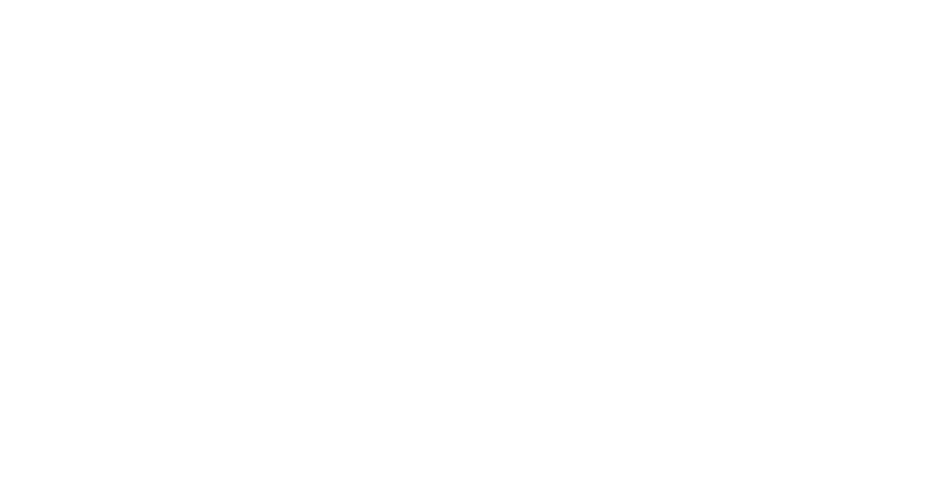
\includegraphics[width=12cm]{AcceleratorLattice-manual-logo.pdf} \\
\vskip 0.3in
\huge\bf David Sagan
\end{center}
}

\vfill
\break


%----------------------------------------------------------------

\cleardoublepage
\phantomsection 
\pdfbookmark[0]{Contents}{Contents}
\pdfbookmark[1]{Table of Contents}{toc} 
\tableofcontents

\cleardoublepage
\phantomsection 
\pdfbookmark[1]{List of Figures}{LoF} 
\listoffigures

\cleardoublepage
\phantomsection 
\pdfbookmark[1]{List of Tables}{LoT} 
\listoftables

%----------------------------------------------------------------
\setlength{\parskip}{\dPar}
\setlength{\parindent}{0ex}

%----------------------------------------------------------------
\part{Overview}
%----------------------------------------------------------------
\chapter{Overview and Introduction}

%---------------------------------------------------------------------------------------------------
\section{acknowledgements}

It is my pleasure to express appreciation to people who have contributed to this effort, and without
whom, \bmadjl would only be a shadow of what it is today: 

\'Etienne Forest (aka Patrice Nishikawa),
Matthew Signorelli,
Alexander Coxe,
Oleksii Beznosov,
Ryan Foussel,
Auralee Edelen,
Chris Mayes,
Georg Hoffstaetter,
Juan Pablo Gonzalez-Aguilera,
Scott Berg,
Dan Abell,
Laurent Deniau,
Hugo Slepicka



%---------------------------------------------------------------------------------------------------
\section{What is Bmad?}

The original Bmad was developed as a subroutine
library ("toolkit") for charged--particle and X-Ray simulations in accelerators and storage rings and 
has served as the calculational engine
for many accelerator simulation programs including the \tao program which is widely used in the
accelerator community. \bmad has
been developed at the Cornell Laboratory for Accelerator-based ScienceS and Education (CLASSE) and
has been in use since 1996.
Eventually in 2023, the organic growth of Bmad --- leading to the code not being as well structured
as it should be --- pushed the decision that the code needed to be
refactored. On top of this was the realization that, while the modern Fortran object-orientated
language that \bmad was written in was a reasonable choice from a purely technical standpoint, 
the Fortran community had atrophied to the point where Fortran compiler maintenance was severely 
affected. The choice was made to use the \julia language for the rewrite.

The name ``\bmad" thus has several meanings. Originally, the term only referred to the \bmad
toolkit. As time went on, and \bmad was used in more and more programs, the term \bmad was
applied to mean the whole ecosystem of toolkit plus programs. Finally, there is the refactored \julia
\bmad. This \bmad is more akin to \bmad-the-ecosystem as
opposed to \bmad-the-toolkit in that \bmad-the-Julia is used both for constructing lattices
(like \bmad-the-toolkit) and for simulation work without an intermediate program interfacing in between.

%---------------------------------------------------------------------------------------------------
\section{History}

\bmad (Otherwise known as ``Baby MAD" or ``Better MAD" or just plain ``Be MAD!") was originally created as
a subroutine
library for charged--particle and X-Ray simulations in accelerators and storage rings. \bmad has
been developed at the Cornell Laboratory for Accelerator-based ScienceS and Education (CLASSE) and
has been in use since 1996.

Prior to the development of \bmad, simulation programs at Cornell were written almost from scratch
to perform calculations that were beyond the capability of existing, generally available software.
This practice was inefficient, leading to much duplication of effort. Since the development of
simulation programs was time consuming, needed calculations where not being done. As a response, the
\bmad subroutine library, using an object oriented approach and written in modern object-oriented
Fortran, were developed. The aim of the \bmad project was to:
\begin{Itemize}
\item Cut down on the time needed to develop programs.
\item Cut down on programming errors.
\item Provide a simple mechanism for lattice function calculations
from within control system programs.
\item Provide a flexible and powerful lattice input format.
\item Standardize sharing of lattice information between 
programs.
\end{Itemize}

\bmad can be used to study both single and multi--particle beam dynamics as well as X-rays.  Over
the years, \bmad modules have been developed for simulating a wide variety of phenomena including
intra beam scattering (IBS), coherent synchrotron radiation (CSR), Wakefields, Touschek scattering,
higher order mode (HOM) resonances, etc., etc.  \bmad has various tracking algorithms including
Runge--Kutta and symplectic (Lie algebraic) integration. Wakefields, and radiation excitation and
damping can be simulated. \bmad has routines for calculating transfer matrices, emittances, Twiss
parameters, dispersion, coupling, etc. The elements that \bmad knows about include quadrupoles, RF
cavities (both storage ring and LINAC accelerating types), solenoids, dipole bends, Bragg crystals
etc.  In addition, elements can be defined to control the attributes of other elements. This can be
used to simulate the ``girder'' which physically support components in the accelerator or to easily
simulate the action of control room ``knobs'' that gang together, say, the current going through a
set of quadrupoles.

%---------------------------------------------------------------------------------------------------
\section{Why Julia?}

The choice of \julia as the basis for the new \bmad was not an easy one. Other possibilities included
C++ \cite{}, Python \cite{}, a combination of Python and C/C++, etc. If the \bmad refactoring
project had been started before 2023 the choice probably would have been Python/C/C++. But in
2023 \julia development was mature enough, and the advantages of \julia over the alternatives was
large enough, so that the decision was made to use \julia.

* Short history of \julia

* \julia was constructed for simulations/large data handling.

* Very active community (not Fortran)

But what is the compelling reason for using \julia? First of all, \julia is a scripting language which
means that it is 
like Python. 

%---------------------------------------------------------------------------------------------------
\section{Manual Organization}

As a consequence of \bmad being a software library, this manual serves two masters: The
programmer who wants to develop applications and needs to know about the inner workings of
\bmad, and the user who simply needs to know about the \bmad standard input format and
about the physics behind the various calculations that \bmad performs.

To this end, this manual is divided into XXX parts. 

Errors and omissions are a fact of life for any
reference work and comments from you, dear reader, are therefore most welcome. Please send
any missives (or chocolates, or any other kind of sustenance) to:
\begin{example}
  David Sagan <dcs16@cornell.edu>
\end{example}

\chapter{Orientation}
\label{c:orient}

\section{What is Bmad?}

\bmad is an open-source software envionment for simulating charged particles and
X-rays. \bmad is not a program itself but is used by programs for doing calculations. The advantage
of \bmad over a stand-alone simulation program is that when new types of simulations need to be
developed, \bmad can be used to cut down on the time needed to develop such programs with the added
benefit that the number of programming errors will be reduced.

Over the years, \bmad has been used for a wide range of charged-particle and X-ray simulations. This
includes:
\begin{example}
Lattice design                                  X-ray simulations
Spin tracking                                   Wakefields and HOMs
Beam breakup (BBU) simulations in ERLs          Touschek Simulations
Intra-beam scattering (IBS) simulations         Dark current tracking
Coherent Synchrotron Radiation (CSR)            Frequency map analysis
\end{example}

%---------------------------------------------------------------------------------------------------
\section{Resources: More Documentation, Obtaining Bmad, etc.}
\label{s:bmad.web}

More information and download instructions are readily available on GitHub:
\begin{example}
  \url{\detokenize{https://github.com/bmad-sim}}
\end{example}

%---------------------------------------------------------------------------------------------------
\section{Type Stability}
\label{s:type.stable}

There is a large amount of information on ``\vn{type stability}'' in Julia so this section will just 
be a short introduction to the subject and the interested reader is urged consult the Julia manual 
as well as the numerous internet articles.

Code is type stable when the Julia compiler can figure out what the type of a variable is at compile
time. For type unstable code, the compiler must add extra stuff to the compiled code to handle the
varias cases that arise when a variable has differing types. For example, with the code
\begin{example}
  a = b * c
\end{example}
the compiled multiplication code will different if \vn{b} and \vn{c} are strings versus integers versus reals, etc.
If the compiler knows the types of \vn{b} and \vn{c}, the execution speed of this code will be much
faster since the compiled code does not have to make any tests as to what the type of \vn{b} and \vn{c}
are. 

It is for this for this reason that ``strongly typed'' languages like C/C++ or Fortran are fast since
the type of all variables must be  declared in the code. A language like Python is slower since 
it is hard for the compiler to infer a variable's type. Julia is in between. Julia can be as fast as
a strongly typed language but only if the programmer takes care to ensure the code is type stable.
How to write code that is type stable is beyond the scope of this introduction and the reader should
consult the literature.

It is important to keep in mind that for code that even without type stability executes quickly and 
will not be executed often, it may not be important that the code be type stable. Indeed,
type stability can come at the price of flexibility and so adherence to type stability is not always warranted.
\include{concepts}

%----------------------------------------------------------------
\part{AcceleratorLattice.jl: Lattice Construction and Manipulation}
%----------------------------------------------------------------
\chapter{Constructing a Lattice}
\label{c:construct-lat}

%---------------------------------------------------------------------------------------------------
\section{Switches}
\label{s:switch}

A \vn{switch} is like an enumerated value except that 


A \vn{switch} is a switch category identifier name, conventionally with the word \vn{Switch} at the end, 
with a set of possible values. Switches are like enums without the associated integer. 
The advantage of switches is that a given switch value can be used for different switch groups. 

For example, 

How to create switches...





%---------------------------------------------------------------------------------------------------
\section{Defining a Lattice Element}
\label{s:ele.def}

The \julia language itself is used as the basis for constructing lattices. Other simulation programs
have similarly utilized the underlying programming language for constructing lattices\cite{merlin++,xsuite},
but this is in marked contrast to such programs as MAD\cite{mad}, Elegant\cite{elegant}, and the 
original \bmad\cite{bmad-orig}. 

Chapter~\sref{c:ele} gives a list of elements defined by \Bmad. Elements are defined using the \vn{@ele}
macro. The general syntax is:
\begin{example}
  @ele eleName = eleType(param1 = val1, param2 = val2, ...)
\end{example}
where \vn{eleName} is the name of the element, \vn{eleType} is the type of element, \vn{param1}, \vn{param2},
etc. are parameter names and \vn{val1}, \vn{val2}, etc. are the parameter values.
Example:
\begin{example}
  @ele qf = Quadrupole(len = 0.6, K1 = 0.370)
\end{example}
The \vn{@ele} macro will construct a \julia variable with the name \vn{eleName}. Additionally the element
that this variable references will also hold \vn{eleName} as the name of the element.

To copy an element use the \vn{deepcopy} constructor.

%---------------------------------------------------------------------------------------------------
\section{Defining a Lattice Element Type}
\label{s:ele.type}

All lattice element types like \vn{Quadrupole}, \vn{Marker}, etc. are subtypes of the abstract type
\vn{Ele}. To construct a new type, use the \vn{\@construct_ele_type} macro. Example:
\begin{example}
  @construct_ele_type MyEleType
\end{example}

%---------------------------------------------------------------------------------------------------
\section{Lattice Element Internals}
\label{s:ele.inside}

All element types have a single component called \vn{pdict} (``parameter dict'') which is of
type \vn{Dict\{Symbol,Any\}}. Using a \vn{Dict} has advantages and disadvantages. The advantage is
that an element is not restricted as to what can be stored in it. The disadvantage is that it is not
type stable (\sref{s:type.stable}). This is generally acceptable when lattices are constructed but
is undesirable during tracking. To regain type stability during tracking, element parameters are
put into immutable structs called \vn{element parameter} groups 
and these structs are stored in \vn{pdict}. During tracking, the tracking
code can access element parameters via the struct which makes the code type stable as will be illustrated below.

The \vn{element parameter} group structures are all subtypes of the abstract type \vn{EleParameterGroup}.
For example, the \vn{LengthGroup} holds the length and s-positions of the element:
\begin{example}
  @kwdef struct LengthGroup <: EleParameterGroup
    L::Float64 = 0
    s::Float64 = 0
    s_downstream::Float64 = 0
  end
\end{example}
The \vn{\@kwdef} macro automatically defines a keyword-based constructor for \vn{LengthGroup}. 
When a parameter group is stored in an element's \vn{pdict}, the key will be the symbol associated
with the struct which in this case is \vn{:LengthGroup}. For example, an element's length can be
accessed via \vn{ele.pdict[:LengthGroup].L}. 


\etcetc...





\chapter{Lattice Elements}
\label{c:elements}
\index{element|hyperbf}

%---------------------------------------------------------------------------------------------------

A lattice is made up of a collection of elements --- quadrupoles,
bends, etc. This chapter discusses the various types of elements
available in \bmad.

\begin{table}[htb]
\centering
{\tt
\begin{tabular}{llll} \toprule
  {\it Element}    & {\it Section}         & {\it Element}      & {\it Section}       \\ \midrule
  BeamBeam         & \ref{s:beambeam}      &  Marker            & \ref{s:mark}        \\ 
  BeginningEle     & \ref{s:begin.ele}     &  Mask              & \ref{s:mask}        \\
  Bend             & \ref{s:bend}          &  Multipole         & \ref{s:mult}        \\
  Collimator       & \ref{s:col}           &  NullEle           & \ref{s:null.ele}    \\
  Converter        & \ref{s:converter}     &  Octupole          & \ref{s:oct}         \\
  CrabCavity       & \ref{s:crab}          &  Patch             & \ref{s:patch}       \\
  Custom           & \ref{s:custom}        &  
  Drift            & \ref{s:drift}         &  Pipe              & \ref{s:monitor}     \\
  EGun             & \ref{s:e.gun}         &  Quadrupole        & \ref{s:quad}        \\
  ElSeparator      & \ref{s:elsep}         &  RFbend            & \ref{s:rf.bend}     \\
  EMField          & \ref{s:em.field}      &  RFcavity          & \ref{s:rfcav}       \\ 
  Fiducial         & \ref{s:fiducial}      &  SadMult           & \ref{s:sad.mult}    \\
  FloorShift       & \ref{s:floor.ele}     &  Sextupole         & \ref{s:sex}         \\
  Foil             & \ref{s:foil}          &  Solenoid          & \ref{s:sol}         \\
  Fork             & \ref{s:fork}          &  Taylor            & \ref{s:taylor}      \\
  Instrument       & \ref{s:monitor}       &  ThickMultipole    & \ref{s:thick.mult}  \\
  Kicker           & \ref{s:kicker}        &  Undulator         & \ref{s:wiggler}     \\
  Lcavity          & \ref{s:lcav}          &  Wiggler           & \ref{s:wiggler}     \\
  \bottomrule
\end{tabular}
} \caption{Table of element types suitable for use with charged particles. Also see
Table~\ref{t:control.classes}} \label{t:particle.classes}
\end{table}

\index{MAD}
Most element types available in \mad are provided in \bmad.  Additionally, \bmad provides a number
of element types that are not available in \mad.  A word of caution: In some cases where both \mad
and \bmad provide the same element type, there will be an overlap of the attributes available but
the two sets of attributes will not be the same.  The list of element types known to \bmad is shown
in Table~\ref{t:particle.classes}, \ref{t:photon.classes}, and \ref{t:control.classes}.
Table~\ref{t:particle.classes} lists the elements suitable for use with charged particles,
Table~\ref{t:photon.classes} which lists the elements suitable for use with photons, and finally
Table~\ref{t:control.classes} lists the \vn{controller} element types that can be used for parameter
control of other elements. Note that some element types are suitable for both particle and photon
use.

\begin{table}[ht]
\centering
{\tt
\begin{tabular}{llll} \toprule
  {\it Element}      & {\it Section}         & {\it Element}         & {\it Section}       \\ \midrule
  Beginning_Ele      & \ref{s:begin.ele}     &    Lens               & \ref{s:lens}        \\
  Capillary          & \ref{s:capillary}     &  Marker               & \ref{s:mark}        \\
  Crystal            & \ref{s:crystal}       &  Mask                 & \ref{s:mask}        \\
  Custom             & \ref{s:custom}        &  Match                & \ref{s:match}       \\
  Detector           & \ref{s:detector}      &  Monitor              & \ref{s:monitor}     \\ 
  Diffraction_Plate  & \ref{s:diff.plate}    &  Mirror               & \ref{s:mirror}      \\
  Drift              & \ref{s:drift}         &  Multilayer_Mirror    & \ref{s:multilayer}  \\
  Ecollimator        & \ref{s:col}           &  Patch                & \ref{s:patch}       \\
  Fiducial           & \ref{s:fiducial}      &  Photon_Fork          & \ref{s:fork}        \\
  Floor_Shift        & \ref{s:floor.ele}     &  Photon_Init          & \ref{s:photon.init} \\
  Fork               & \ref{s:fork}          &  Pipe                 & \ref{s:monitor}     \\
  GKicker            & \ref{s:gkicker}       &  Rcollimator          & \ref{s:col}         \\
  Instrument         & \ref{s:monitor}       &  Sample               & \ref{s:sample}      \\
  \bottomrule
\end{tabular}
}
\caption{Table of element types suitable for use with photons. Also see Table~\ref{t:control.classes}}
\label{t:photon.classes}
\end{table}

\begin{table}[ht]
\centering
{\tt
\begin{tabular}{llll} \toprule
  {\it Element}  & {\it Section}     & {\it Element}  & {\it Section}    \\ \midrule
  Controller     & \ref{s:group}     &  Ramper        & \ref{s:ramper}   \\
  Girder         & \ref{s:girder}    &                &                  \\
 \\ \bottomrule
\end{tabular}
}
\caption{Table of controller elements.}
\label{t:control.classes}
\end{table}

For a listing of element attributes for each type of element, see Chapter~\sref{c:attrib.list}.

\newpage

%---------------------------------------------------------------------------------------------------
\section{Lattice Element Parameters}

Before discussing lattice elements themselves, the element parameters need to be discussed first.
Element parameters are divided into immutable struct groups which inherit from the abstract type
\vn{EleParameterGroup}. A list of parameter groups can be seen using the command

For example, the position of the element with respect

Element parameters are listed in 

%---------------------------------------------------------------------------------------------------
\section{Anatomy of a Lattice Element}

All lattice elements inherit from the abstract type \vn{Ele}. There is a macro \vn{construct_ele_type}
that is used to construct a new type of element. For example:
\begin{example}
  @construct_ele_type Bend
\end{example}
this defines the immutable \vn{Bend} struct which inherits from \vn{Ele}. 

All element structs have a single \vn{Dict\{Symbol,Any\}} field called \vn{param}.
The dot selection operator has been overloaded so that something like \vn{ele.name}
is mapped to \vn{ele.param[:name]}. Except!




%----------------------------------------------------------------
\part{TPSA.jl: Truncated Power Series Algebra}
%----------------------------------------------------------------

%----------------------------------------------------------------
\part{Simulations With Bmad}
%----------------------------------------------------------------

%----------------------------------------------------------------
\part{Conventions and Physics}
%----------------------------------------------------------------

%----------------------------------------------------------------
\part{Bibliography}
%----------------------------------------------------------------

\cleardoublepage
\phantomsection


\end{document}

